The objective of realising an embedded system, able to control via a
SVM model an advanced, dexterous hand prosthesis such as, e.g., Touch
Bionics's i-LIMB is nowadays at hand, thanks to the remarkable degree
of development of microelectronics and micro-controller technology for
prosthetics. Here we sketch a possible architecture for such an
implementation in our framework.

Due to the necessity of small, lightweight and low-power consuming
hardware in this framework, we propose a centralised architecture
based upon a micro-controller such as, e.g., \textbf{EMANUELE}
... \cite{...}. This would minimise the number of required
components. Figure \ref{fig:mc} is a schema of the proposed
architecture.

\begin{figure*}[!ht] \centering
  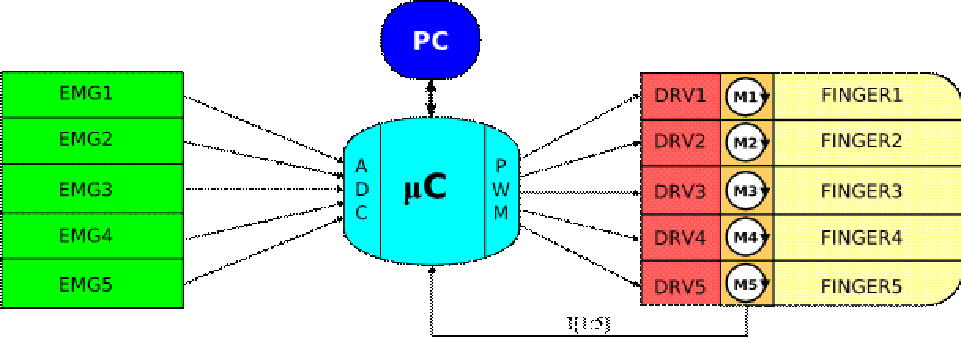
\includegraphics[width=0.9\textwidth]{figs/mc}
  \caption{a schema for the miniaturisation of the proposed method
    onto a micro-controller.}
  \label{fig:mc}
\end{figure*}

In a practical setting, the proposed method operates in two
independent modalities, according to the standard paradigm of
supervised machine learning: \emph{training}, when EMG and force data
are acquired and the related SVM models are built, and
\emph{prediction}, when the models receive ``live'' EMG data and
output the posture / grip indexes and the force required by the
patient. Usually --- and this is the case --- training is a much more
complex and resource-demanding issue than predicting. For now, we
envision that training can be carried out off-line, using additional
hardware such as a force sensor in controlled conditions, and a
dedicated PC. Once the SVM models have been created in the training
phase, they can be transferred onboard the micro-controller via the
connection visible in the above Figure. Therefore, the tasks the
micro-controller is supposed to perform are essentially:

\begin{enumerate}

  \item the live, real-time acquisition of the EMG signals and of
    current signals coming from the motors of the prosthesis;

  \item the prediction of the required posture / grip and force;

  \item the motor control, realised via PWM signals based upon the
    prediction of the previous step;

  \item the communication with the off-line PC, at least as far as
    $(a)$ upload of hyperparameters and models and $(b)$ exchange of
    general system information for stastical purposes are concerned;

  \item safety management.

\end{enumerate}

An ADC device, mounted onboard the micro-controller, takes care of
acquiring the signals. This is an easy task, since the EMG maximum
required sampling rate would not exceed $25$Hz as is clear from the
previous Sections. As well, there is no filtering / envelope /
root-mean-square evaluation burden, since the Otto Bock electrodes
already perform these task. Current feedback signals, at least one per
motor, can as well be acquired easilty, as is done in standard
myoelectric prosthetics.

The posture / grip indexes required by the patient must be translated
to appropriate position control signals, to be sent to the motor
controllers; the required force can be enforced, as an initial
possibility, as a proportional torque at the hand joints, that is, a
current applied to each motor, according to the simple relationship $I
= K_M M$, where $K_M$ is the motor's torque-to-current conversion
factor. A more sophisticated schema could enforce \emph{impedance
control} at the hand (see, e.g., \cite{alin}) if the hand itself is
dexterous and sophisticated enough to allow it. The motors are
actuated using a PWM signal per each motor, managed by the
micro-contorller. For the associated power motor drivers, a standard
H-bridge schema would suffice. \textbf{EMANUELE}

Besides the SVM models, the micro-controller will store, e.g., the
maximum safety values for the motor currents and the PWM controllers
duty-cycles; the PC connection could in this case be used as well to
monitor the behaviour of the system. As well, the system must provide
patient-independent emergency control routines to manage dangerous
situations, such as, e.g., the low-battery conditions.
